% This work is licensed under the Creative Commons Attribution-NonCommercial 4.0 International License.
% To view a copy of this license, visit http://creativecommons.org/licenses/by-nc/4.0/
% or send a letter to Creative Commons, PO Box 1866, Mountain View, CA 94042, USA.

% !TEX TS-program = xelatex

\documentclass[../Main/chem532-notes.tex]{subfiles}

\setcounter{chapter}{1}
\begin{document}

\chapter{H\"{u}ckel Theory}

\section{Foundation of the H\"{u}ckel MO Method}
H\"{u}ckel molecular orbital theory is one of the simplest methods to determine the energy of $\pi$ electrons in conjugated organic molecules. This approach neglects the $\sigma$ electrons and makes several simplifications in the treatment of the $\pi$ electrons.
%Consider only $\pi$ electrons of conjugated hydrocarbons.   Assume that the orbital (MO) each electron occupies is expressed as linear combination of atomic orbitals (LCAO).

\begin{example}[ethylene, 2 electrons / 2 orbitals]
The simplest problem that can be solved with the H\"{u}ckel method is the ethylene molecule. For each carbon we describe the electrons in the C 2p$_z$ using one basis function ($\chi_1$ and $\chi_2$)
\begin{center}
\includegraphics[width =1in]{../huckel/ethylene_mos.png}
\end{center}
\end{example}

\begin{example}[benzene, 6 electrons / 6 orbitals]
In the case of benzene, the H\"{u}ckel method only describes electrons in the C 2p$_z$ responsible for $\pi$ bonding
\begin{center}
\includegraphics[width =1in]{../huckel/benzene_mos.png}
\end{center}
\end{example}

In the H\"{u}ckel method electrons occupy molecular orbitals (MOs), $\psi_i(\mathbf{r})$, that are written as a linear combination of atomic orbitals (LCAO).
The $i$-th molecular orbital $\psi_i(\mathbf{r})$ is written as
\begin{equation}
\psi_i(\mathbf{r}) = \sum_\mu^{N} \chi_\mu(\mathbf{r}) C_{\mu i},
\end{equation}
where:
\begin{itemize}
\item  $N$ is the number of atomic orbitals (AOs) = number of molecular orbitals (MOs) = number of atoms that share p$_z$ orbitals
\item  the functions $\chi_\mu(\mathbf{r}): \mathbb{R}^3 \rightarrow \mathbb{R}$ are atomic p$_z$ orbitals (also called basis functions)
\item  $\mathbf{r} = (x,y,z)$ is the electron coordinate (we will neglect spin for now)
\item the matrix $\mathbf{C}$ with elements $(\mathbf{C})_{\mu i} = C_{\mu i}$ gives the coefficient of the $\mu$-th AO in the $i$-th MO. In other words, read the coefficient of $\psi_i$ from the $i$-th column of the matrix $\mathbf{C}$.
\end{itemize}

\begin{example}
The MOs of ethylene are written as $\psi_i(r) = \chi_1(r) C_{1 i} + \chi_2(r) C_{2 i}$.
\end{example}

H\"{u}ckel theory postulates that the MOs satisfy the following Schr\"{o}dinger equation:
\begin{equation}
\label{eq:huckel:schrodinger equation}
\hat{h}(1) \psi_i(1) = \epsilon_i \psi_i(1),
\end{equation}
where
\begin{itemize}
\item $\hat{h}(1)$ is an effective one-electron Hamiltonian
\item $\epsilon_i$ is energy of the $i$-th MO
\item $(1) = (x_1,y_1,z_1)$ collects the space coordinate of an electron
\end{itemize}

The H\"{u}ckel one-electron Hamiltonian is expressed as
\begin{equation}
\hat{h}(1) = \hat{T}(1) + \hat{V}(1),
\end{equation}
where $\hat{T}(1)$ is the kinetic energy operator
\begin{equation}
\hat{T}(1) = -\frac{\hbar^2}{2 m}\left( \frac{\partial^2}{\partial x_1^2} + \frac{\partial^2}{\partial y_1^2} + \frac{\partial^2}{\partial z_1^2} \right),
\end{equation}
and $\hat{V}(1)$ is an ``effective'' potential energy for an electron.
In H\"{u}ckel we do not assume that $\hat{V}(1)$ is known. All the integrals that enter in the theory are parameters that are adjusted to match experiment.

It is convenient to introduce the following integrals in the AO basis:
\begin{align}
h_{\mu \mu} = & \bra{\chi_\mu} \hat{h} \ket{\chi_\mu} =   \int d\mathbf{r} \, \chi_\mu^* \hat{h}(\mathbf{r}) \chi_\mu(\mathbf{r})  \quad \text{(Coulomb integral of AO $\mu$)} \\
h_{\mu \nu} = & \bra{\chi_\mu} \hat{h} \ket{\chi_\nu} =  \int d\mathbf{r} \, \chi_\mu^*(\mathbf{r}) \hat{h} \chi_\nu(\mathbf{r}) \quad \text{(Resonance integral between AOs $\mu$ and $\nu$)} \\
S_{\mu \nu} = &  \braket{\chi_\mu | \chi_\nu} =  \int d\mathbf{r} \,  \chi_\mu^*(\mathbf{r}) \chi_\nu(\mathbf{r}) d\mathbf{r} \quad \text{(Overlap integral between AOs $\mu$ and $\nu$)}
\end{align}

\section{Determination of the MO coefficients}
To determine the MO orbitals we insert the definition $\ket{\psi_i} = \sum_\mu^{N} \ket{\chi_\mu} C_{\mu i}$ into the Schr\"{o}dinger equation [Eq.~\eqref{eq:huckel:schrodinger equation}] 

\begin{equation}
\hat{h}(1) \sum_\mu^{N} \ket{ \chi_\mu} C_{\mu i}= \epsilon_i \sum_\mu^{N} \ket{ \chi_\mu} C_{\mu i},
\end{equation}
Multiply by $\bra{\chi_\nu}$ from the left.  The left hand side becomes:
\begin{equation}
\bra{\chi_\nu}\hat{h}(1) \sum_\mu^{N} \ket{ \chi_\mu} C_{\mu i}
=  \sum_\mu^{N}  \bra{\chi_\nu}\hat{h}(1)\ket{ \chi_\mu} C_{\mu i} =  \sum_\mu^{N}  h_{\nu\mu} C_{\mu i}
\end{equation}
The right hand side is:
\begin{equation}
\bra{\chi_\nu}\epsilon_i \sum_\mu^{N} \ket{ \chi_\mu} C_{\mu i} = 
\sum_\mu^{N} \braket{\chi_\nu|\chi_\mu} C_{\mu i}  \epsilon_i 
= \sum_\mu^{N}S_{\nu\mu} C_{\mu i}  \epsilon_i 
\end{equation}

Therefore we have:
\begin{equation}
\sum_\mu^{N}  h_{\nu\mu} C_{\mu i} = \sum_\mu^{N}S_{\nu\mu} C_{\mu i}  \epsilon_i,
\end{equation}
which in matrix notation reads:

\begin{equation}
\begin{pmatrix}
h_{11} & h_{12} & \ldots & h_{1N} \\
h_{21} & h_{22} & \ldots & h_{2N} \\
\vdots & \vdots & \ddots & \vdots \\
h_{N1} & h_{N2} & \ldots & h_{NN} \\
\end{pmatrix}
\begin{pmatrix}
C_{1i} \\
C_{2i} \\
\vdots \\
C_{Ni}
\end{pmatrix}
= 
\begin{pmatrix}
S_{11} & S_{12} & \ldots & S_{1N} \\
S_{21} & S_{22} & \ldots & S_{2N} \\
\vdots & \vdots & \ddots & \vdots \\
S_{N1} & S_{N2} & \ldots & S_{NN} \\
\end{pmatrix}
\begin{pmatrix}
C_{1i} \\
C_{2i} \\
\vdots \\
C_{Ni}
\end{pmatrix}
\epsilon_i,
%\sum_\mu^{N}  h_{\nu\mu} C_{\mu i} = \sum_\mu^{N}S_{\nu\mu} C_{\mu i}  \epsilon_i,
\end{equation}
or more compactly:
\begin{equation} \label{eq:eigensystem}
\mathbf{H} \mathbf{c}_i = \mathbf{S} \mathbf{c}_i \epsilon_i,
\end{equation}
where $\mathbf{c}_i$ is the column matrix 
\begin{equation}
\mathbf{c}_i = 
\begin{pmatrix}
C_{1i} \\
C_{2i} \\
\vdots \\
C_{Ni}
\end{pmatrix}.
\end{equation}
If we combine all the columns together into the matrix $\mathbf{C} = (\mathbf{c}_1, \mathbf{c}_2, \ldots, \mathbf{c}_N)$, we can write Eq.~\eqref{eq:eigensystem} as
\begin{equation} \label{eq:eigensystem_matrix}
\mathbf{H} \mathbf{C} = \mathbf{S} \mathbf{C} \boldsymbol{\epsilon},
\end{equation}
where the matrix $\boldsymbol{\epsilon}$ contains all the orbital energies in the diagonal elements
\begin{equation}
\boldsymbol{\epsilon} = \begin{pmatrix}
\epsilon_{1} &0 & \ldots & 0 \\
0 & \epsilon_{2} & \ldots & 0 \\
\vdots & \vdots & \ddots & \vdots \\
0 & 0 & \ldots & \epsilon_{N} \\
\end{pmatrix}
\end{equation}



\begin{problem}	
Convince yourself that Eq.~\ref{eq:eigensystem_matrix} is correct.
\end{problem}

The H\"{u}ckel method for conjugated hydrocarbons further \textbf{assumes}:
\begin{itemize}
\item $h_{\mu\mu} = \alpha < 0$ (same for all carbon atoms), where $\alpha$ is the energy of an electron in AO $\chi_\mu \approx - I_{\mu}$  (ionization energy)
\item $h_{\mu\nu} =
\begin{cases} \beta < 0 \quad \text{if $\mu$ and $\nu$ are on adjacent atoms}\\
0 \quad \text{otherwise}
\end{cases}$

$|\beta|$ measures the strength of interaction between AOs $\mu$ and $\nu$ and it is a negative quantity.

\item That we neglect the overlap of atomic orbitals. This means that atomic orbitals are normalized ($\braket{\chi_\mu | \chi_\mu} = 1$) and orthogonal ($\braket{\chi_\mu | \chi_\nu} = 0$ if $\mu \neq \nu$).
This implies that the overlap matrix $\mathbf{S}$ is the identity matrix, that is, $S_{\mu\nu} = \delta_{\mu\nu} = \begin{cases}1 \quad \text{if } \mu = \nu\\
0 \quad \text{if } \mu \neq \nu
\end{cases}$ .
%	      = 0 (otherwise)
%h_{\nu\mu} C_{\mu i} = \sum_\mu^{N}S_{\nu\mu} C_{\mu i}  \epsilon_i,
\end{itemize}

\section{The H\"{u}ckel Method in Practice}
\begin{example}[Ethylene]

The Hamiltonian in the H\"{u}ckel approximation is:
\begin{equation}
\mathbf{H} = \begin{pmatrix}
\alpha & \beta \\
\beta & \alpha
\end{pmatrix}
\end{equation}

The Schr\"{o}dinger equation reads:
\begin{equation}
\begin{pmatrix}
\alpha & \beta \\
\beta & \alpha
\end{pmatrix}
\begin{pmatrix}
C_{1i}\\
C_{2i}
\end{pmatrix}
=
\begin{pmatrix}
1 & 0 \\
0 & 1
\end{pmatrix}
\begin{pmatrix}
C_{1i}\\
C_{2i}
\end{pmatrix}
\epsilon_i
\end{equation}
Simplify and rearrange:
\begin{equation}
\begin{pmatrix}
\alpha - \epsilon_i & \beta \\
\beta & \alpha - \epsilon_i
\end{pmatrix}
\begin{pmatrix}
C_{1i}\\
C_{2i}
\end{pmatrix}
= 0
\end{equation}
This equation has non-trivial solutions
A trivial solution to a linear system $\mathbf{A}\mathbf{x} = \mathbf{0}$ is the solution $\mathbf{x} = \mathbf{0}$. In this example the trivial solution is $\begin{pmatrix}
C_{1i}\\
C_{2i}
\end{pmatrix} = 
\begin{pmatrix}
0\\
0
\end{pmatrix}$
only if the determinant of the secular matrix is equal to zero:
\begin{equation}
\begin{vmatrix}
\alpha - \epsilon_i & \beta \\
\beta & \alpha - \epsilon_i
\end{vmatrix}
= 0
\Rightarrow
\beta^2 \begin{vmatrix}
\frac{\alpha - \epsilon_i}{\beta} & 1 \\
1 & \frac{\alpha - \epsilon_i}{\beta}
\end{vmatrix}
= 0
\end{equation}

Introduce the reduced variable $\frac{\alpha - \epsilon_i}{\beta} = - \lambda$ and evaluate the secular determinant:

\begin{equation}
\begin{vmatrix}
\frac{\alpha - \epsilon_i}{\beta} & 1 \\
1 & \frac{\alpha - \epsilon_i}{\beta}
\end{vmatrix}
= \begin{vmatrix}
-\lambda & 1 \\
1 & -\lambda
\end{vmatrix}
= \lambda^2 - 1 = 0,
\end{equation}
from this equation we obtain the eigenvalues:
\begin{equation}
\lambda^2 = \left(\frac{\alpha - \epsilon_i}{\beta}\right)^2 = 1
\Rightarrow
\frac{\alpha - \epsilon_i}{\beta} = \pm 1
\Rightarrow
\epsilon_i = \alpha \pm \beta
\end{equation}

\begin{center}
\includegraphics[width = 2in]{../huckel/c2_ethylene_1.png}
\end{center}

\end{example}

\begin{example}[Butadiene]
Note that cis-butadiene and trans-butadiene are the same in Hückel MOs.
\begin{center}
\includegraphics[width = 4in]{../huckel/c2_butadiene.png}
\end{center}

\end{example}

\begin{example}[Benzene]
The Hamiltonian in the H\"{u}ckel approximation is:

\begin{equation}
\mathbf{H}
=
\begin{pmatrix}
\alpha & \beta & & & & \beta\\
\beta & \alpha & \beta & & & \\
& \beta & \alpha & \beta & & \\
& & \beta & \alpha & \beta & \\
& & & \beta & \alpha & \beta \\
\beta  & & & & \beta & \alpha \\
\end{pmatrix}
\end{equation}
\end{example}

You only need the ``connectivity'' of a molecule to write down the H\"{u}ckel Hamiltonian.

\begin{problem}
Write down the H\"{u}ckel Hamiltonian for:
\begin{enumerate}
\item butadiene
\item naphthalene
\item azulene
\end{enumerate}
\end{problem}

%\begin{example}[H\"{u}ckel computation on butadiene]
%The following shows the energy and coefficient matrix for butadiene. 
%\begin{verbatim}
% Energies
%        1      2(HOMO)   3(LUMO)   4
%       1.618034   .618034  -.618034 -1.618034    MO energies
%
%MO coefficients
%    0   .371748  -.601501   .601501  -.371748    AO1
%    1   .601501  -.371748  -.371748   .601501    AO2
%    2   .601501   .371748  -.371748  -.601501    AO3
%    3   .371748   .601501   .601501   .371748    AO4
%         MO1       MO2       MO3       MO4
%\end{verbatim}
%MO1 and MO4 are paired, and MO2 and MO3 are paired.
%Do not forget that the sign of MO as a whole is arbitrary.  i.e. $\phi_i$ or $-\phi_i$ are both OK.
%\end{example}

In the H\"{u}ckel method, the energy is given by the sum of the orbital energies ($\epsilon_i$) of all the occupied orbitals
\begin{equation}
E = \sum_i \epsilon_i n_i,
\end{equation}
where $n_i$ is the occupation number of the orbital $i$. This quantity can be 0, 1, or 2
\begin{equation}
n_i \in \{0, 1, 2 \}.
\end{equation}

Note that some times the eigenvalues are also expressed in the following form
\begin{equation}
\epsilon_i = \alpha + \lambda_i \beta,
\end{equation}
in terms of the reduced variable $\lambda_i$.




\section{Heteroatoms}

For hydrocarbons containing heteroatoms we introduce atom-specific and bond-specific matrix elements.
\begin{example}[Acrolein]

In the case of acrolein we define modified H\"{u}ckel parameters:
\begin{itemize}
\item $\alpha_{\rm O} = \alpha + 2 \beta$	(O is more electronegative than C)
\item $\beta_{\rm CO} = \sqrt{2} \beta$	(C = 0 $\pi$ bond is shorter and stronger than C=C)
\item $\alpha_{\rm C'} = \alpha + 0.2 \beta$	(C of CO is slightly more electronegative due to C$\rightarrow$O charge transfer)
\end{itemize}

\begin{center}
\includegraphics[width = 1in]{../huckel/c2_acrolein.png}
\end{center}
The H\"{u}ckel Hamiltonian for acrolein is
\begin{equation}
\mathbf{H}
=
\begin{pmatrix}
\alpha & \beta & & \\
\beta & \alpha & \beta & \\
& \beta & \alpha + 0.2 \beta & \sqrt{2} \beta \\
& &  \sqrt{2} \beta & \alpha + 2 \beta \\
\end{pmatrix}.
\end{equation}

\end{example}



\begin{table}[h!]
   \centering
   \caption{Recommended values of the parameters for heteroatoms in the H\"{u}ckel method} % requires the topcapt package
   \begin{tabular}{@{} lcllcl @{}} % Column formatting, @{} suppresses leading/trailing space
      \toprule
	\multicolumn{3}{c}{Diagonal elements} & \multicolumn{3}{c}{Off-diagonal elements} \\
	\midrule
	\multicolumn{3}{c}{Coulomb Integrals} & \multicolumn{3}{c}{Resonance Integrals}\\
	\multicolumn{3}{c}{$\alpha_{\rm X} = \alpha_{\rm C} + l_{\rm X} \beta_{\rm CC}$}
	& \multicolumn{3}{c}{$\beta_{\rm XY} = k_{\rm XY} \beta_{\rm CC}$}\\
	\midrule
	atom X & \# of $\pi$ electrons & $l_{\rm X}$ & atom X-Y & \# of $\pi$ electrons & $k_{\rm XY}$ \\
	\midrule
	= C -- & (1) & 0.0 & C--C & (1-1) & 1.0 \\
	= N -- & (1) & 0.5 & C = N & (1-1) & 1.1 \\
	- N:< & (2) & 0.8 & C $\equiv$ N & (1-1) & 1.3 \\
	- O - & (1) & 1.1 & C--N: & (1-2) & 0.9 \\
	- O: & (2) & 1.5 & C = O & (1-1) & 1.2 \\
	- F: & (2) & 2.0 & C--O: & (1-2) & 0.7 \\
	- Cl: & (2) & 1.7 & C = S & (1-1) & 1.0 \\
	- Br: & (2) & 1.3 & C--S: & (1-2) & 0.5 \\
	- I: & (2) & 1.15 & C--F & (1-2) & 0.95 \\
	= S & (1) & 0.3 & C--Cl & (1-2) & 0.7 \\
	- S: & (2) & 1.0 & C--I & (1-2) & 0.5 \\
	& & & N = N & (1-1) & 1.2\\
	& & & N--O & (2-1) & 1.1 \\
	\\
	\multicolumn{6}{c}{Hyperconjugated methyl group (CH$_3$)}  \\
	C & (1) & $-$0.1 &  C $\equiv$ H$_3$ & (1-1) & 2.5   \\
	H$_3$ & (1) & $-$0.5 & C--CH$_3$ & (1-1) & 0.6\\
	\bottomrule
   \end{tabular}
   
   Larger $l_{\rm X}$, more electronegative the atom X. Larger $k_{\rm XY}$, stronger the bond XY.
   \label{tab:booktabs}
\end{table}

\section{Pairing Theorem for Alternant Hydrocarbons (AHs)}
For alternant hydrocarbons (hydrocarbons without odd-membered rings), MO energies are paired, which means that they are symmetric with respect to the energy $\alpha$\mnote{Recall that $\frac{\alpha - \epsilon_i}{\beta} = - \lambda_i$.}
\begin{align}
\epsilon_i &= \alpha + \lambda_i \beta, \\
\epsilon_{N - i + 1} &= \alpha - \lambda_i \beta.
\end{align}

\begin{example}[Pairing theorem for ethylene, butadiene, and benzene]
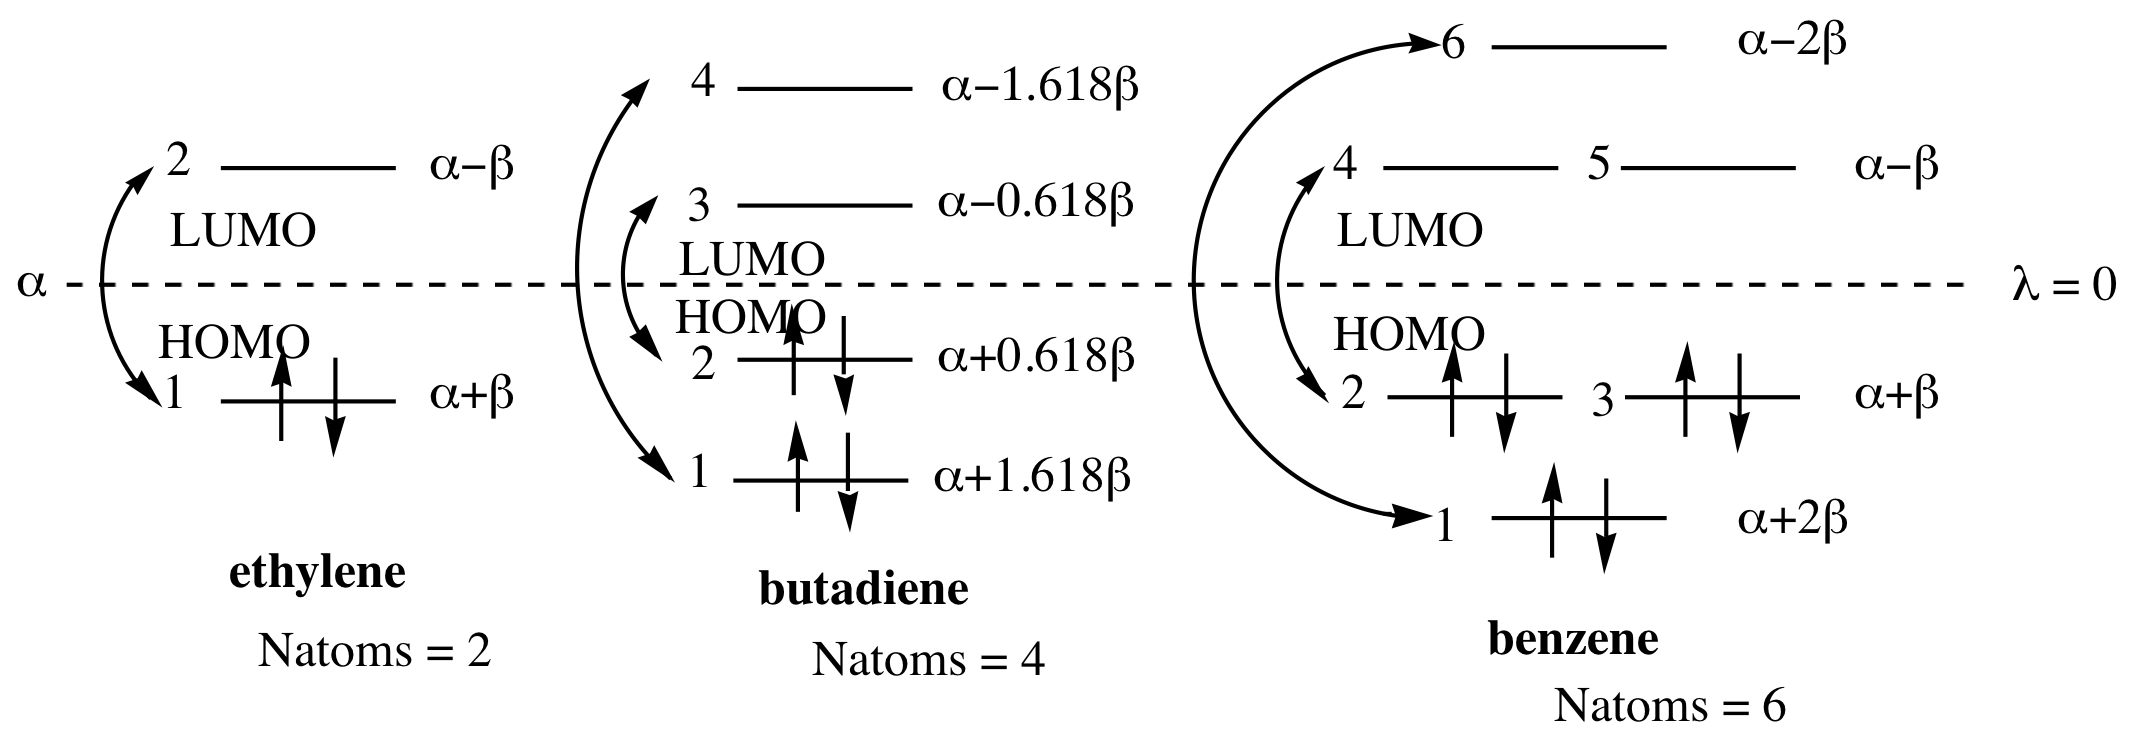
\includegraphics[width = 5in]{../huckel/c2_pairing_theorem.png}
\end{example}

An interesting implication is that alternant hydrocarbons with an odd number of carbons have an orbital with $\lambda_i = 0$, that is $\epsilon_i = \alpha$.
To see this consider the case $N = 2k + 1$ and consider the level $i = k + 1$. In this case the energy $\epsilon_{k + 1}$ is equal to that of $\epsilon_{N - (k + 1) + 1}$, from which we obtain
\begin{align}
\epsilon_{k + 1} = \epsilon_{N - (k + 1) + 1} \Rightarrow \alpha + \lambda_i \beta=  \alpha - \lambda_i \beta  \Rightarrow \lambda_i = 0.
\end{align}

\begin{example}[Pairing theorem for the allyl and benzyl radicals (odd alternant)]
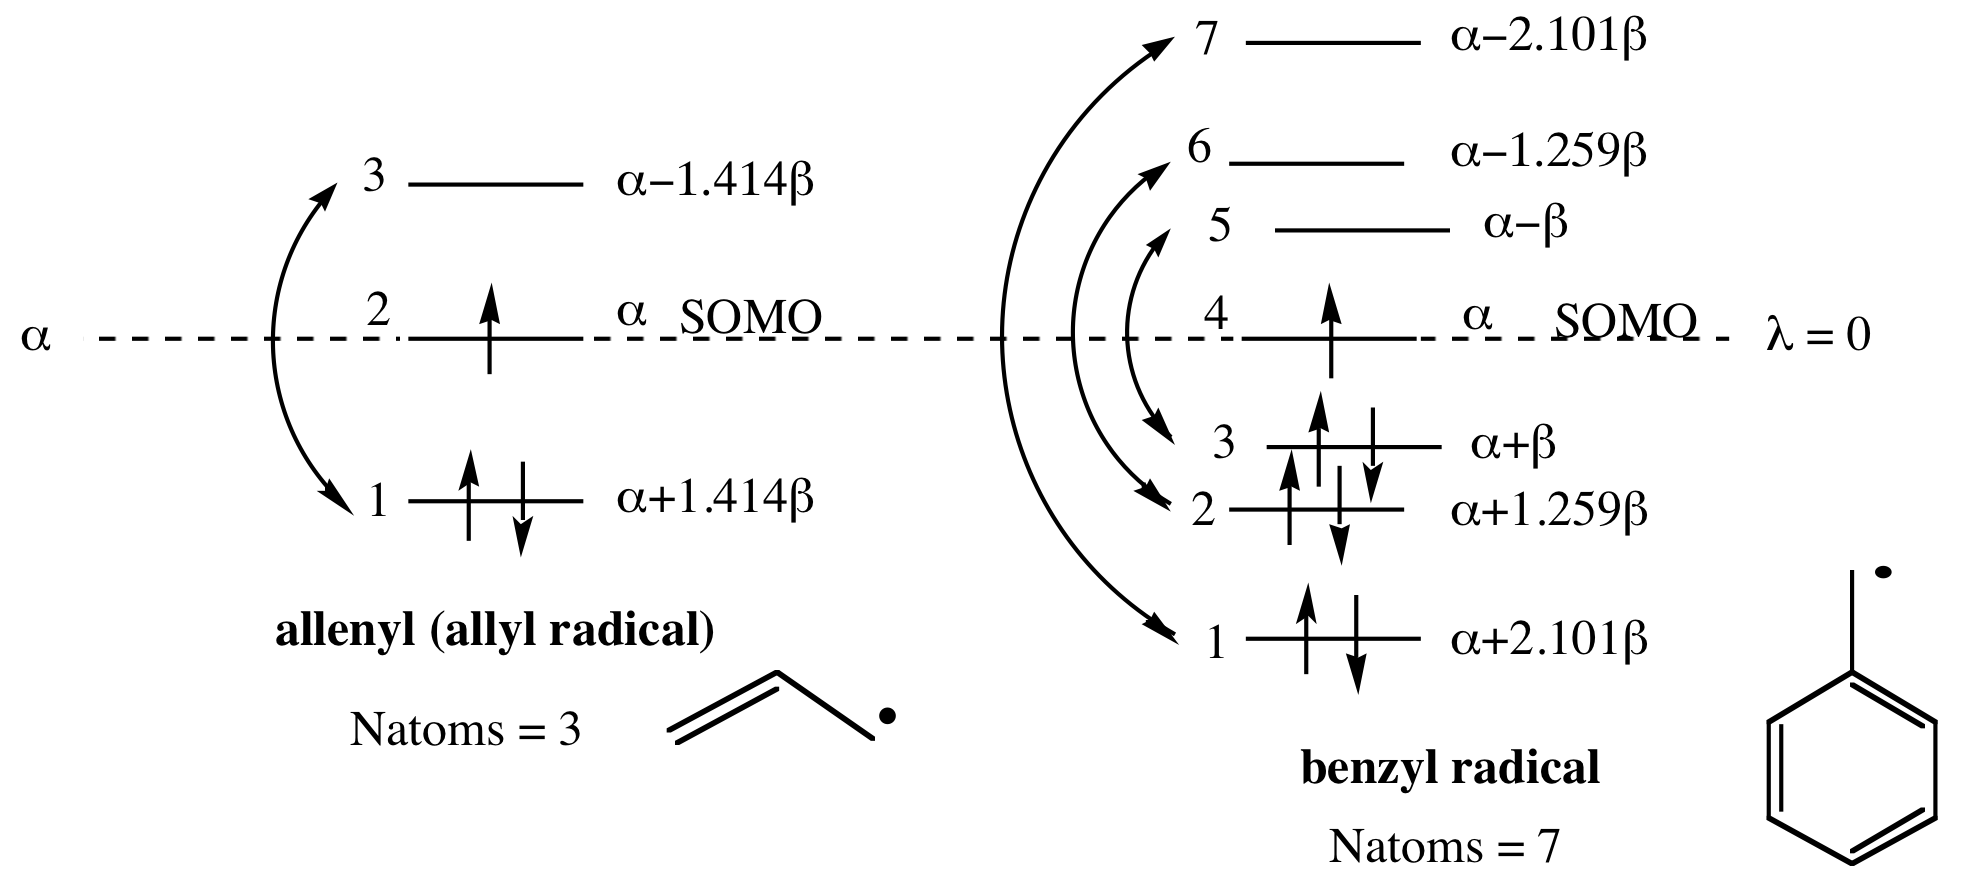
\includegraphics[width = 5in]{../huckel/c2_pairing_theorem2.png}

In the allyl radical the second MO ($\psi_2$, $\epsilon_2 = \alpha$) is paired to itself. In the benzyl radical the fourth MO ($\psi_4$, $\epsilon_4 = \alpha$) is paired to itself.
\end{example}

\begin{example}[Non alternant hydrocarbons]
In this example, the energies of the cyclopropenyl cation are not paired

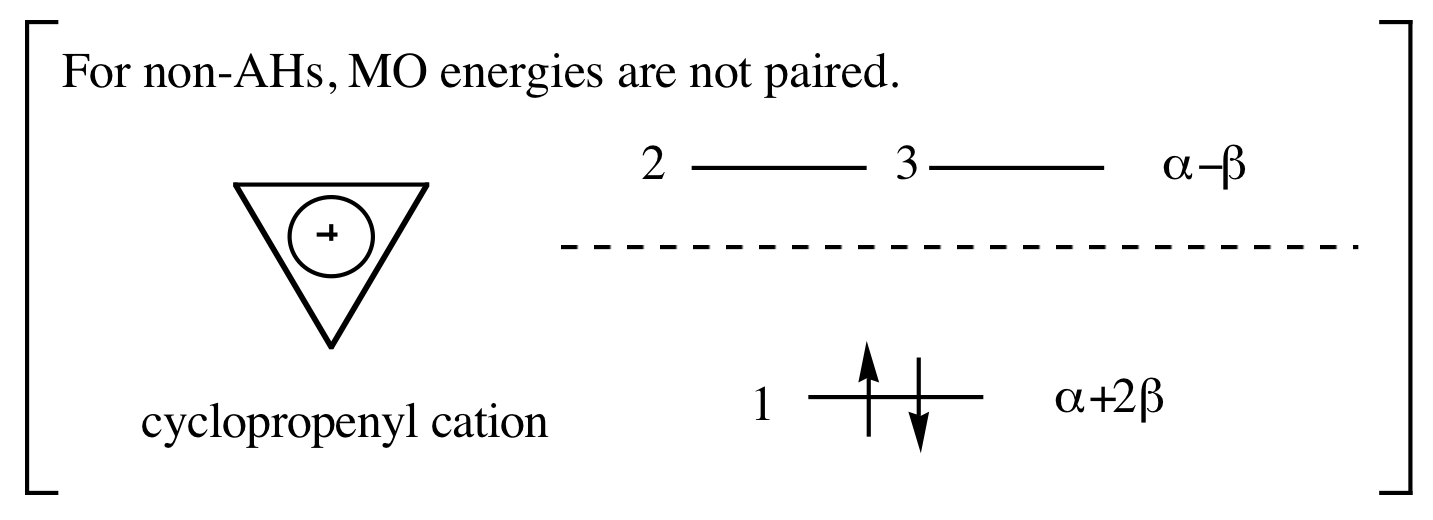
\includegraphics[width = 3in]{../huckel/c2_nonalternant.png}
\end{example}



Another consequence of this theorem is that the coefficients of paired orbitals are also paired (MOs $\psi_i$ and $\psi_{N-i+1}$ are paired). This property is best expressed by labeling alternating carbon atoms with a star (*) and the relationship
\begin{align}
C_{\mu, N - i + 1} &= \;\;\;C_{\mu i} \quad \text{ when $\mu$ = starred atom} \\
&= - C_{\mu i}  \quad \text{ when $\mu$ = unstarred atom}.
\end{align}

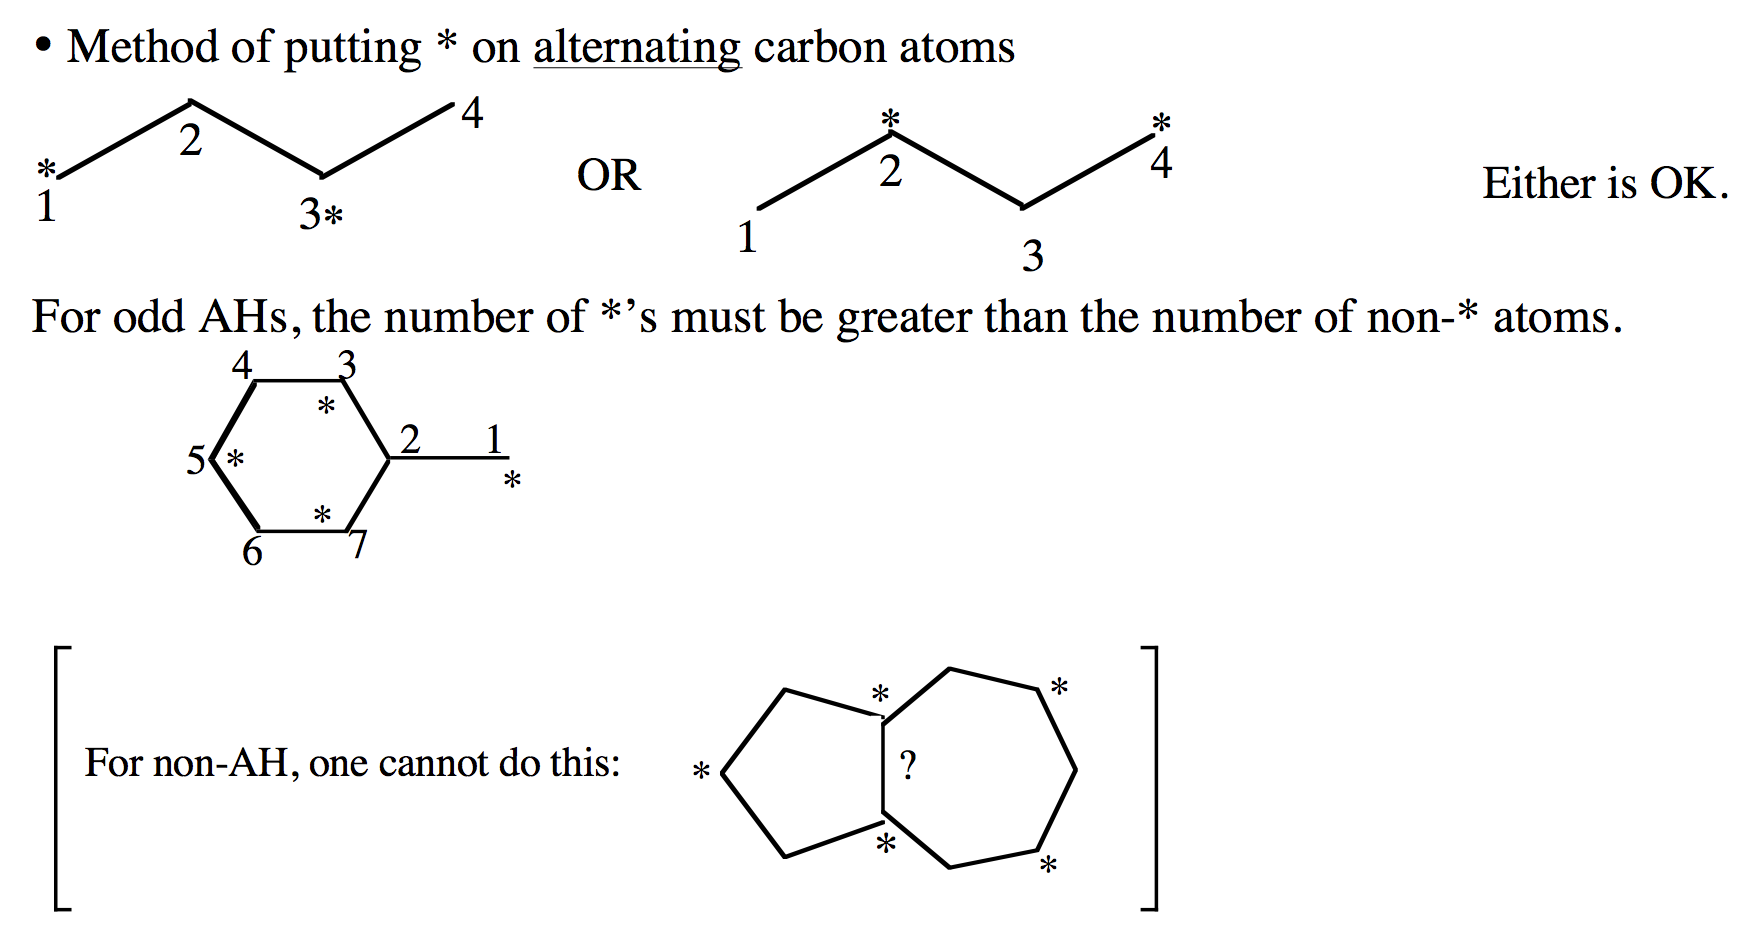
\includegraphics[width = 5in]{../huckel/c2_alternant.png}

\begin{example}[H\"{u}ckel computation on butadiene]
The following shows the energy and coefficient matrix for butadiene. 
\begin{verbatim}
 Energies
        1         2(HOMO)   3(LUMO)   4
       1.618034   .618034  -.618034 -1.618034    MO energies

MO coefficients
    0   .371748  -.601501   .601501  -.371748    <- AO1
    1   .601501  -.371748  -.371748   .601501    <- AO2
    2   .601501   .371748  -.371748  -.601501    <- AO3
    3   .371748   .601501   .601501   .371748    <- AO4
         MO1       MO2       MO3       MO4
\end{verbatim}
Note that the energies and coefficients of MOs 1 and 4 and MOs 2 and 3 are paired.
Do not forget that the sign of MO as a whole is arbitrary.  i.e. $\psi_i$ or $-\psi_i$ are both OK.
\end{example}

\begin{example}[H\"{u}ckel computation on allyl radical]
The following shows the energy and coefficient matrix for the allyl radical. 
\begin{verbatim}
 Energies
        1       2(SOMO)   3(LUMO) 
       1.414214 .000000 -1.414214    MO energies

MO coefficients
    0   -.500000 -.707107   .500000    <- AO1
    1   -.707107  .000000  -.707107    <- AO2
    2   -.500000  .707107   .500000    <- AO3
         MO1       MO2       MO3

DENSITY AND BOND ORDER MATRIX
         1        2         3 
    1   1.000000
    2    .707107 1.000000
    3    .000000  .707107  1.000000
         
DEGENERACIES: HOMO=0 LUMO = 0 TOTAL ENERGY = 3 ALPHA + 2.828427 BETA         
\end{verbatim}
Note that the energies and coefficients of MOs 1 and 3 are paired.
\end{example}

When MOs are degenerate (i.e., two MOs have same energy), their MO coefficients can not be uniquely determined.  Any linear combination of degenerate MOs is also acceptable MO of the same energy.  Appropriate transformation among degenerate MOs is needed to show pairing.

\section{Symmetry of MOs}
Each MO is symmetric or antisymmetric with respect to symmetry operations of the system.

\begin{example}[Symmetry of the orbitals in butadiene]
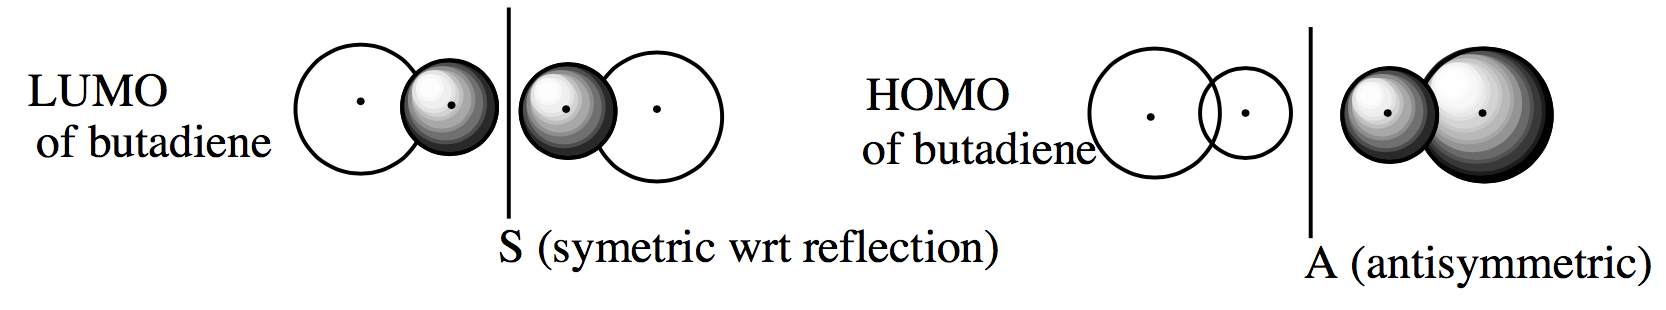
\includegraphics[width=4in]{../huckel/c2_symmetry_ex1.png}
\end{example}

\begin{example}[Symmetry of the orbitals in the allyl radical]
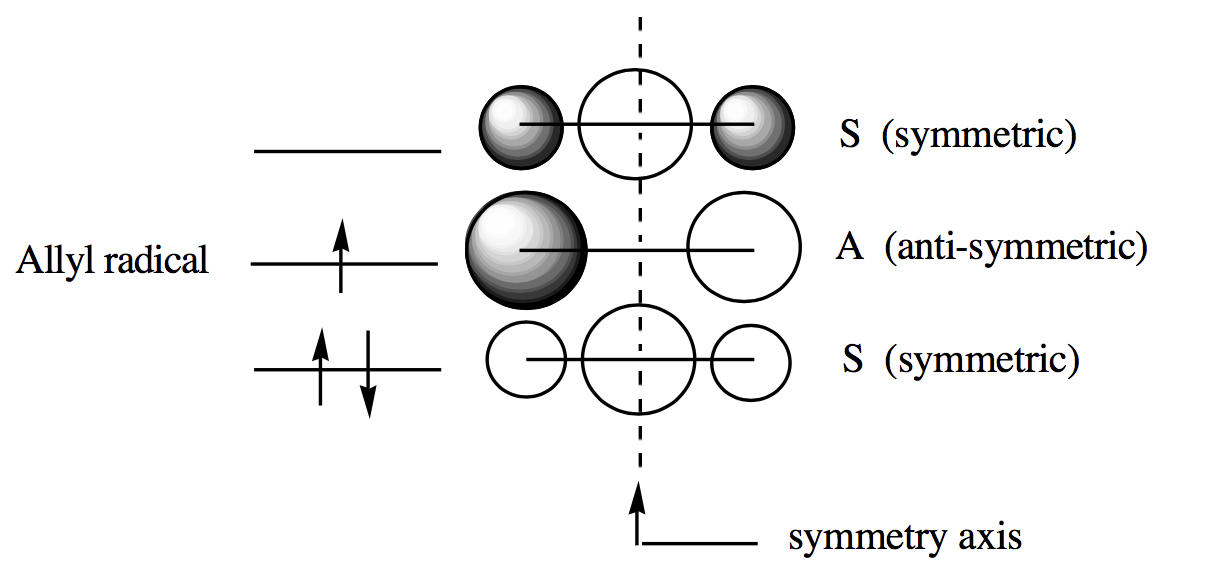
\includegraphics[width=3in]{../huckel/c2_symmetry_ex2.png}
\end{example}

\begin{example}[Symmetry of the orbitals in benzene]
This example shows that when MOs are degenerate, appropriate linear combinations of degenerate MOs can be made to satisfy symmetry.

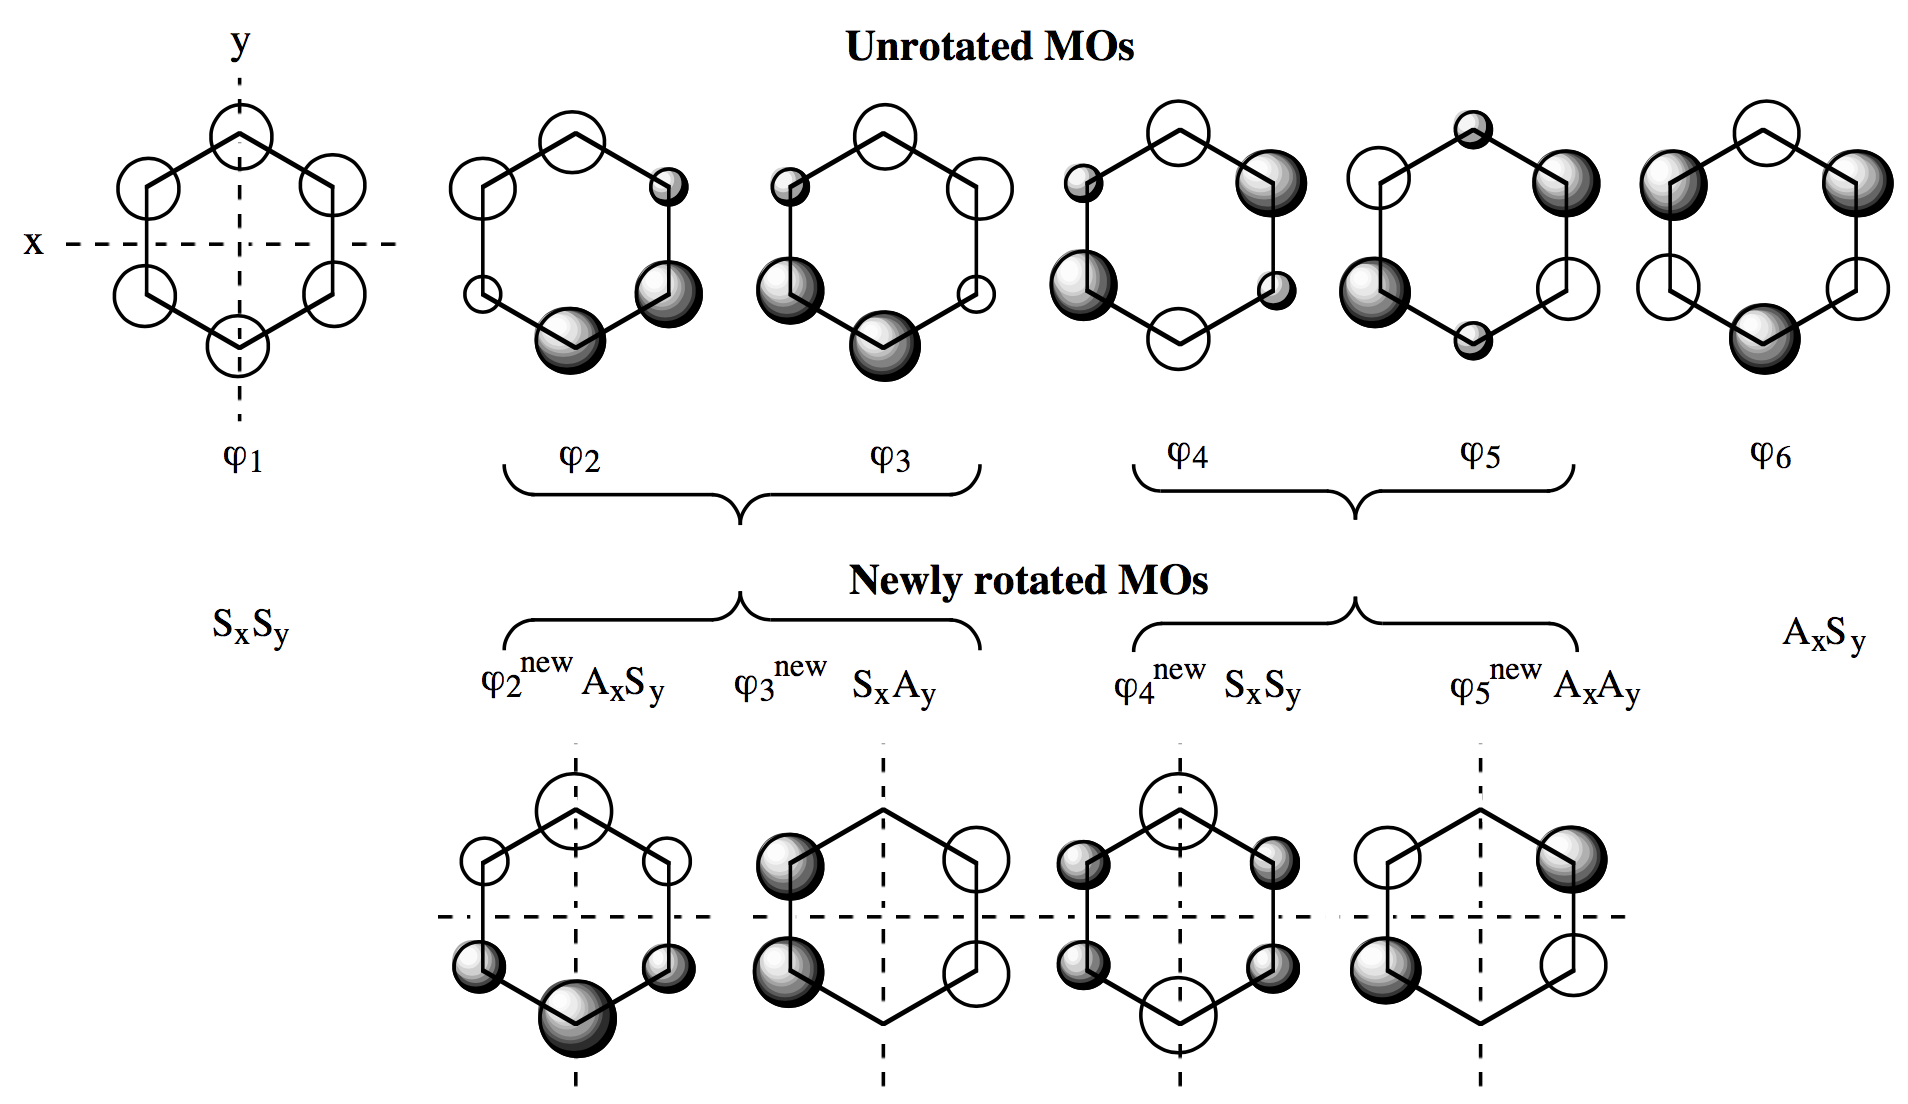
\includegraphics[width=4.5in]{../huckel/c2_symmetry_ex3.png}

In this example, the MOs of the benzene molecule were transformed according to
\begin{align*}
\psi_2^\mathrm{new} & = +\cos \theta \psi_2 + \sin \theta \psi_3  \\
\psi_3^\mathrm{new} & = -\sin \theta \psi_2 + \cos \theta \psi_3 
\end{align*}
and chosen either to be such that $|C_{12}|$ is maximized, which in this case is also equivalent to $C_{13} = 0$.
\begin{verbatim}
 Energies
         1         2         3         4         5         6
        2.000000  1.000000  1.000000 -1.000000 -1.000000 -2.000000

 MO coefficients

    1   .408248   .455142   .355218   .567622  -.105541  -.408248
    2   .408248   .535198  -.216555  -.192409   .544345   .408248
    3   .408248   .080057  -.571773  -.375212  -.438804  -.408248
    4   .408248  -.455142  -.355218   .567622  -.105541   .408248
    5   .408248  -.535198   .216555  -.192409   .544345  -.408248
    6   .408248  -.080057   .571773  -.375212  -.438804   .408248
           1         2         3         4         5         6

 New Energies
        1         2         3         4         5         6
       2.000000  1.000000  1.000000 -1.000000 -1.000000 -2.000000

 New MO coefficients
    1   .408248   .577350   .000000   .577350   .000000  -.408248
    2   .408248   .288675  -.500000  -.288675   .500000   .408248
    3   .408248  -.288675  -.500000  -.288675  -.500000  -.408248
    4   .408248  -.577350   .000000   .577350   .000000   .408248
    5   .408248  -.288675   .500000  -.288675   .500000  -.408248
    6   .408248   .288675   .500000  -.288675  -.500000   .408248
           1         2         3         4         5         6

 DEGENERACIES:  HOMO=  2    LUMO=  2
\end{verbatim}
Shown above are two sets of orbitals for benzene. Note that orbitals 2 and 3 and 4 and 5 are degenerate. Therefore, we are allowed to separately mix them without changing the orbital energies.
\end{example}

%\section{NBMO (Non-bonding MO) back-of-the-envelope calculation}
%
%Once a wise man said: ``For odd alternant hydrocarbon radicals, the SOMO (Singly Occupied MO, $\lambda_i$=0) can be calculated by hand''.
%
%This is a consequence of the pairing theorem for odd alternant hydrocarbon. Recall that the $\mu$-th row of the secular equation for the SOMO and $\mu$ = a non-starred atom is given by:
%\begin{equation}
%C_{\sigma_1 i} - \lambda_i C_{\mu i} + C_{\sigma_2 i} + C_{\sigma_3 i} = 0,
%\quad 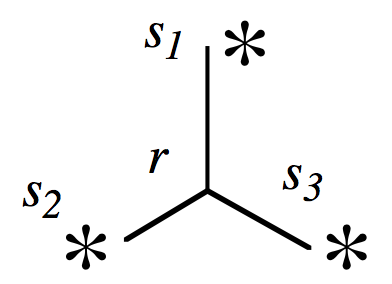
\includegraphics[width=1in]{../huckel/c2_nbmo_1.png}
%\end{equation}
%where $\sigma_j$ stands for a surrounding starred atom.
%Since for the SOMO we have that $\lambda_i = 0$ then it follows that
%\begin{equation}
%\sum_{\sigma}^{\text{neighbors of non *atom}} C_{\sigma i} = 0.
%\end{equation}
%
%\begin{example}[Allyl radical]
%For the allyl radical we can easily compute the SOMO
%
%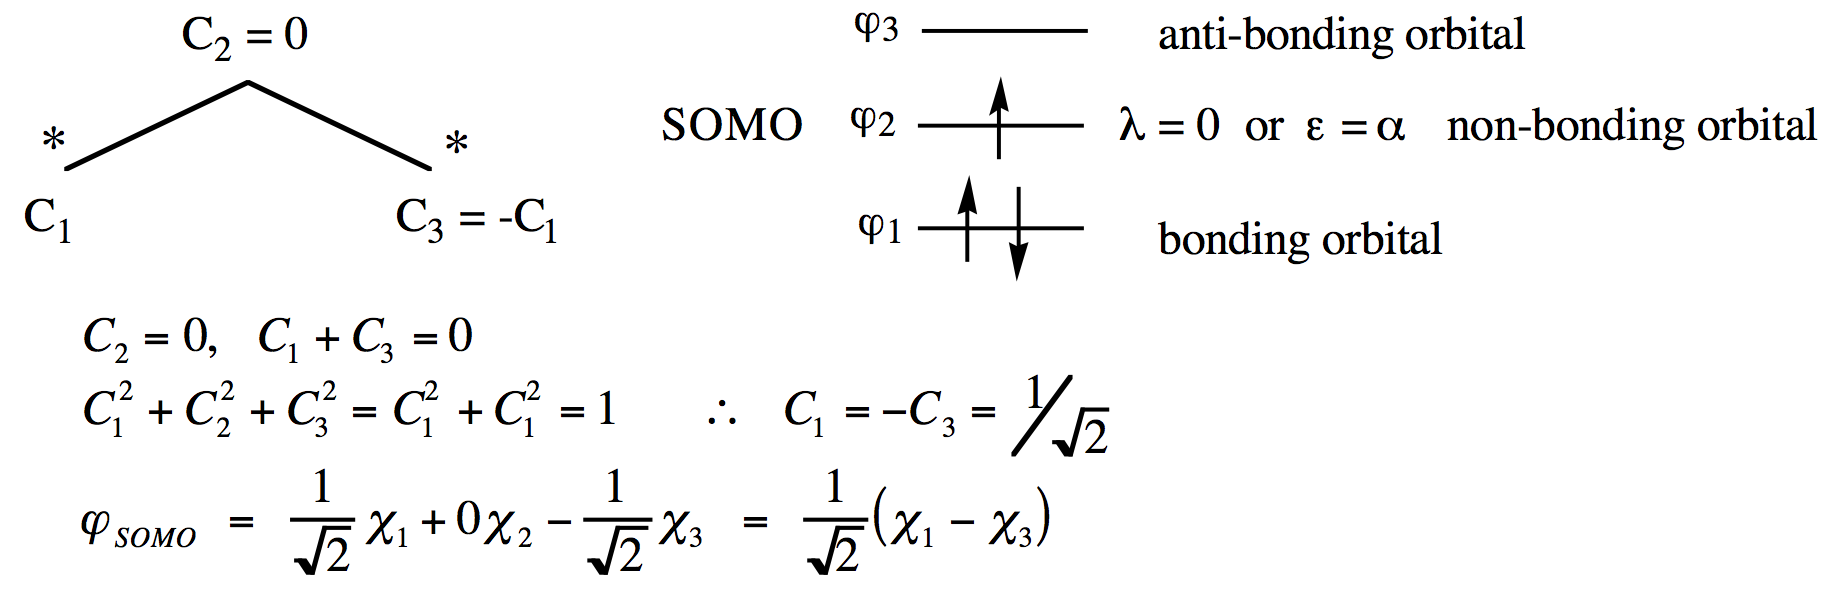
\includegraphics[width=4.5in]{../huckel/c2_nbmo_ex1.png}
%
%\end{example}
%
%\begin{example}[Benzyl radical] We can evaluate the reactivity
%
%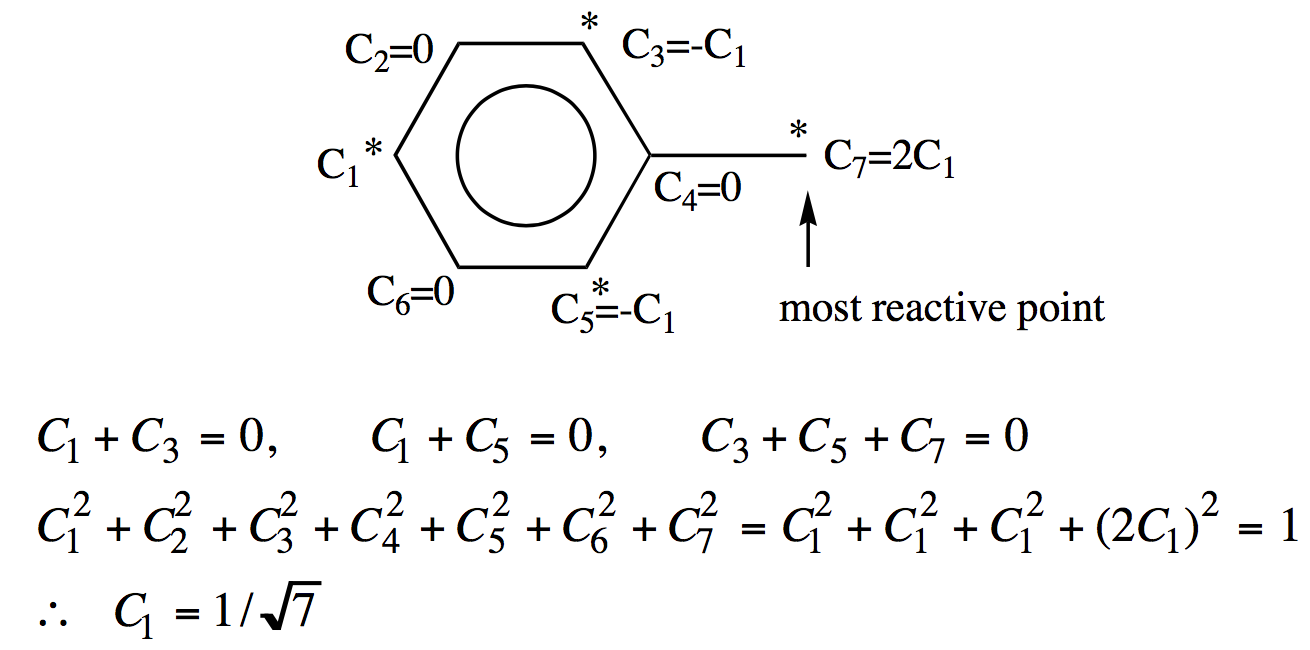
\includegraphics[width=3in]{../huckel/c2_nbmo_ex2.png}
%
%\end{example}
%	
%What is this good for:
%\begin{enumerate}
%\item Showing off.
%\item Predict the qualitative spin density distribution. (exp. measured by ESR)
%\item Predict the qualitative reactivity of radicals.
%\end{enumerate}
%
%\begin{example}[Further examples] Consider the following molecules:
%
%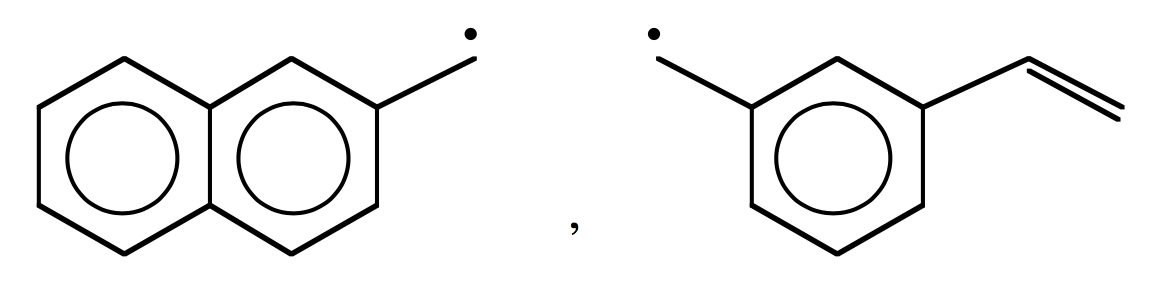
\includegraphics[width=3in]{../huckel/c2_nbmo_ex3.png}
%\end{example}

\section{MO electron density and bond order, total electron density and total bond order}
Recall that $i$-th MO can be expanded in terms of the AOs ($\chi_\mu$ = AO) and the coefficient matrix ($C_{\mu i}$) as:
\begin{equation}
\psi_i = \sum_\mu^{N} \chi_\mu C_{\mu i}.
\end{equation}
Since each MO is normalized we can write:\mnote{Recall that in quantum mechanics $|\Psi|^2 = \Psi^* \Psi$ is a probability density.}
\begin{equation}
\begin{split}
1 = & \braket{\psi_i | \psi_i} = 
\sum_{\mu \nu}^N C_{\mu i}^*  \underbrace{\braket{\chi_\mu | \chi_\nu}}_{S_{\mu\nu}} C_{\nu i}
= \sum_{\mu}^N C_{\mu i}^* C_{\mu i}  S_{\mu\mu}
+ \sum_{\mu}^N \sum_{\substack{\nu\\ \nu \neq \mu}}^N C_{\mu i}^* C_{\nu i}  S_{\mu\nu} \\
= & \sum_{\mu} |C_{\mu i}|^2 + \sum_{\mu \neq \nu} C_{\mu i}^* C_{\nu i}  S_{\mu\nu}.
\end{split}
\end{equation}
\mnote{To simplify the notation we will write $\sum_{\mu} \sum_{\substack{\nu\\ \nu \neq \mu}}$ as $\sum_{\mu \neq \nu}$ and omit the superscript $N$.}
We can interpret the last two terms in the following way
\begin{itemize}
\item $q^i_\mu = |C_{\mu i}|^2$ is the probability of finding an electron in MO $\psi_i$ on the atomic orbital $\chi_\mu$. Therefore, we call this the \textbf{electron density} on AO $\chi_\mu$ due to the MO $\psi_i$.

\item $p_{\mu \nu}^i = C_{\mu i}^* C_{\nu i}$ may be interpreted as the \textbf{bond order} for bond $\mu$-$\nu$ in MO $\psi_i$ (recall that the H\"{u}ckel method assumes $S_{\mu\nu} = 0$ when $\mu \neq \nu$).
\end{itemize}

\begin{example}[Electron density for the first and second MOs of the allyl radical]

\begin{center}
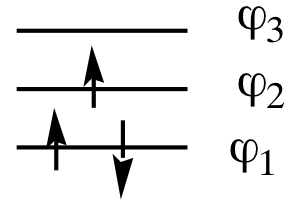
\includegraphics[width=1in]{../huckel/c2_allyl_ediagram.png}
\end{center}

For $\psi_1$
\begin{center}
\begin{tabular}{@{} lcr @{}} % Column formatting, @{} suppresses leading/trailing space
\toprule
AO & MO Coefficient ($C_{\mu i}$) & Electron density ($q^i_\mu = |C_{\mu i}|^2$)\\
\midrule
1 & $C_{11} = -0.5$ & $q_{1}^{1} = 0.25$ \\
2 & $C_{21} = -0.7071$ & $q_{2}^{1} = 0.5$ \\
3 & $C_{31} = -0.5$ & $q_{3}^{1} = 0.25$ \\
\midrule
Sum & & $\displaystyle \sum_{\mu = 1}^{N} q^1_\mu = 1.0$ \\
\bottomrule
\end{tabular}
\end{center}

For $\psi_2$
\begin{center}
\begin{tabular}{@{} lcr @{}} % Column formatting, @{} suppresses leading/trailing space
\toprule
AO & MO Coefficient ($C_{\mu i}$) & Electron density ($q^i_\mu = |C_{\mu i}|^2$)\\
\midrule
1 & $C_{12} = 0.7071$ & $q_{1}^{2} = 0.5$ \\
2 & $C_{22} = 0$ & $q_{2}^{2} = 0$ \\
3 & $C_{32} = -0.7071$ & $q_{3}^{2} = 0.5$ \\
\midrule
Sum & & $\displaystyle \sum_{\mu = 1}^{N} q^2_\mu = 1.0$ \\
\bottomrule
\end{tabular}
\end{center}
\end{example}


Using these quantities we define:
\begin{itemize}
\item \textbf{Total density on atom} $\mu$ ($q_\mu$):
\begin{equation}
q_\mu = \sum_{i}^{\rm MO} n_i |C_{\mu i}|^2 = \sum_{i}^{\rm MO} n_i q_\mu^i \quad n_i \text{ = occupation (2, 1, or 0)} 
\end{equation}

\item \textbf{Total charge on atom} $\mu$ ($N_\mu$):
\begin{equation}
N_\mu = (\text{number of $\pi$ electrons donated by atom $\mu$}) - q_\mu
\end{equation}

\item \textbf{Total bond order between atoms  $\mu$ and  $\nu$} ($p_{\mu \nu}$):
\begin{equation}
p_{\mu \nu}= \sum_{i}^{\rm MO} n_i C_{\mu i}^* C_{\nu i} = \sum_{i}^{\rm MO} n_i p_{\mu\nu}^i
\end{equation}
\end{itemize}

Note that the orbital energy may be rewritten using the orbital density ($q^i_\mu = |C_{\mu i}|^2$) and bond order ($p_{\mu \nu}^i = C_{\mu i}^* C_{\nu i}$)
\begin{equation}
\epsilon_i = \braket{\psi_i | \hat{h} | \psi_i} = \sum_{\mu} q_{\mu}^{i} \alpha_{\mu} + 2 \sum_{\mu <  \nu} p_{\mu \nu}^i \beta_{\mu\nu}.
\end{equation}
and the total energy can be also expressed using the total density and bond order as
\begin{equation}
E = \sum_i^\mathrm{occ} n_i \epsilon_i = \sum_{\mu} q_{\mu} \alpha_{\mu} + 2 \sum_{\mu < \nu} p_{\mu \nu} \beta_{\mu\nu}.
\end{equation}

\begin{example}[H\"{u}ckel computation on allyl radical]
The following shows the density and bond order matrix for the allyl radical. 
\begin{verbatim}
Density and bond order matrix
         1         2         3 
    1   1.000000  0.707107  0.000000
    2   0.707107  1.000000  0.707107
    3   0.000000  0.707107  1.000000
\end{verbatim}

\begin{center}
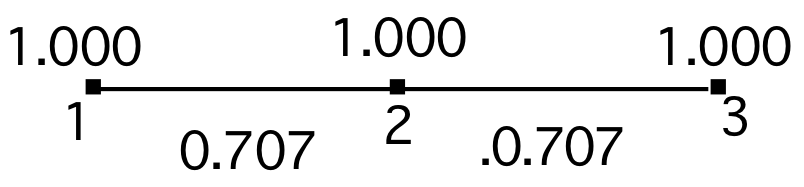
\includegraphics[width=2in]{../huckel/c2_allyl_bond_order.png}
\end{center}

\begin{equation}
p_{12} = 2 C_{11} C_{21} +  C_{12} C_{22} = 2 \times 0.5 \times (-0.7071) + 0.7071 \times 0 = 0.7071.
\end{equation}

Note that for alternant hydrocarbons the pairing theorem always gives $q_\mu = 1$.
\end{example}

\begin{example}[H\"{u}ckel computation on butadiene]
The following shows the density and bond order matrix for butadiene. 
\begin{verbatim}
Density and bond order matrix
         1         2         3         4 
    1   1.000000  0.894427  0.000000 -0.447214
    2   0.894427  1.000000  0.447214  0.000000
    3   0.000000  0.447214  1.000000  0.894427
    4  -0.447214  0.000000  0.894427  1.000000
\end{verbatim}

Note that the 1-2 and 3-4 bonds ($p_{12} = p_{34} = 0.894427$) are stronger than the 2-3 bond ($p_{23} = 0.447214$). Also, ignore the negative values for non-nearneighbor atoms.
\end{example}

\begin{example}[H\"{u}ckel computation on pyridine]
The following shows a full H\"{u}ckel computation for pyridine. 
\begin{verbatim}
 NATOMS  NELECS  NINDEX   NLAB   NHOMO   NLUMO
    6       6       0       1       3       4

 Input Matrix
       1       2       3       4       5       6
    1   .5000
    2  1.1000   .0000
    3   .0000  1.0000   .0000
    4   .0000   .0000  1.0000   .0000
    5   .0000   .0000   .0000  1.0000   .0000
    6  1.1000   .0000   .0000   .0000  1.0000   .0000

 Energies
    1         2         3         4         5         6
   2.199322  1.206641  1.000000  -.916933 -1.000000 -1.989029
 
 MO coefficients 
    1   .558416   .525891   .000000   .528265   .000000  -.364069
    2   .431331   .168916   .500000  -.340234   .500000   .411900
    3   .334378  -.374659   .500000  -.269119  -.500000  -.418804
    4   .304074  -.620995   .000000   .586999   .000000   .421114
    5   .334378  -.374659  -.500000  -.269119   .500000  -.418804
    6   .431331   .168916  -.500000  -.340234  -.500000   .411900
    
 Total energy = 6 ALPHA +  8.811924 BETA

 Density and bond-order matrix
        1          2         3         4         5         6
    1  1.176780 
    2  0.659388   0.929159
    3 -0.020615   0.661883  1.004356
    4 -0.313552   0.052521  0.668674  0.956191
    5 -0.020615  -0.338117  0.004356  0.668674  1.004356
    6  0.659388  -0.070841  -.338117  0.052521  0.661883  0.929159

 Total charges:
	N1: 1 - 1.177= -0.177
	C2: 1 - 0.929= +0.071
	C3: 1 - 1.004= -0.104
	C4: 1 - 0.956= +0.044
\end{verbatim}
\end{example}

\begin{example}[H\"{u}ckel computation on pyrrole]
The following shows a full H\"{u}ckel computation for pyrrole. 
\begin{verbatim}
NATOMS  NELECS  NINDEX   NLAB   NHOMO   NLUMO
    5       6       0       1       3       4

 Input Matrix
       1       2       3       4       5
    1   .8000
    2   .9000   .0000
    3   .0000  1.0000   .0000
    4   .0000   .0000  1.0000   .0000
    5   .9000   .0000   .0000  1.0000   .0000

 Energies
         1         2         3         4         5
       2.120048   .920296   .618034 -1.240344 -1.618034

 MO coefficients
    1  -.583903  -.643479   .000000   .494968   .000000
    2  -.428211  -.043004  -.601501  -.561058  -.371748
    3  -.382315   .539554  -.371748   .250434   .601501
    4  -.382315   .539554   .371748   .250434  -.601501
    5  -.428211  -.043004   .601501  -.561058   .371748

 Total energy = 6 ALPHA +  7.316756 BETA

 Density and bond-order matrix
          1         2         3         4         5
    1  1.510014
    2   .555412  1.094034
    3  -.247914   .728230  1.150959
    4  -.247914  -.166198   .598172  1.150959
    5   .555412  -.353179  -.166198   .728230  1.094034

 Total charges:
    N1: 2 - 1.510= +0.490
    C2: 1 - 1.094= -0.094
    C3: 1 - 1.151= -0.151
\end{verbatim}
\end{example}

\section{Orbital Interactions and Symmetry}
H\"{u}ckel theory can be used to qualitatively understand how the interaction of orbitals leads to the stabilization or destabilization intermediate species formed during a chemical reaction.
To estimate the interaction of a molecule with a reagent (R) use second order perturbation theory.
Consider the case of an electrophile reagent (R) that interacts with atom $\mu$ of a given molecule. In H\"{u}ckel theory the matrix element corresponding to this interaction can be represented with a scaled version of the resonance integral $\beta$
\begin{equation}
\braket{\chi_\mu | \hat{h}'| \chi_R} = \gamma \beta,
\end{equation}
where $0 \leq \gamma <1$ is a parameter that describes the strength of this interaction.

\begin{center}
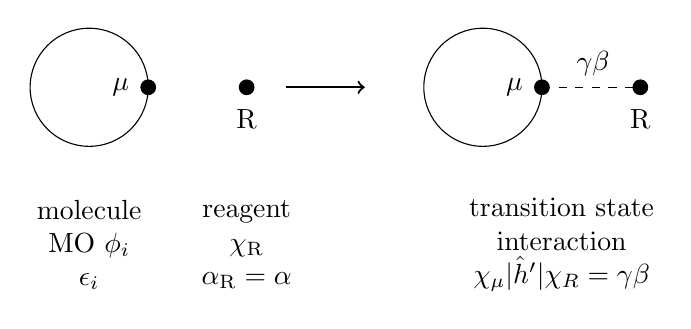
\begin{tikzpicture}
\draw (2,2) circle (0.75);
\fill[black] (2.75,2) circle (0.1);
\node at (2.4,2) {$\mu$};
\fill[black] (4,2) circle (0.1);
\node at (4,1.6) {R};
\draw[thick,->] (4.5,2) -- (5.5,2);
\draw (7,2) circle (0.75);
\fill[black] (7.75,2) circle (0.1);
\node at (7.4,2) {$\mu$};
\draw[dashed] (7.75,2) -- (9,2);
\fill[black] (9,2) circle (0.1);
\node at (9,1.6) {R};
\node at (8.4,2.3) {$\gamma\beta$};
\node[align=center] at (2,0) {molecule\\ MO $\phi_i$ \\$\epsilon_i$};
\node[align=center] at (4,0) {reagent\\ $\chi_\mathrm{R}$\\$\alpha_\mathrm{R} = \alpha$};
\node[align=center] at (8,0) {transition state \\ interaction \\ $\braket{\chi_\mu | \hat{h}'| \chi_R} = \gamma \beta$};
\end{tikzpicture}
\end{center}

%Recall that the second-order perturbation energy correction of the energy for an orbital $\psi_i$ due to a perturbation $\hat{h}'$ is given by
%\begin{equation}
%\Delta E_i^{(2)} = \sum_{k \neq i}^\text{unoccupied states} \frac{|\braket{\psi_i|\hat{h}'|\psi_k}|^2}{\epsilon_i - \epsilon_k},
%\end{equation}
%where $\hat{h}'$ contains the terms that describe the interaction between A and B.


Each  molecular orbital $\psi_i$ from H\"{u}ckel theory gets stabilized by an energy amount given by
\begin{equation}
\Delta E_i^{(2)} = \frac{|\braket{\psi_i|\hat{h}'|\chi_R}|^2}{\epsilon_i - \epsilon_R}.
\end{equation}
Note that there is no summation here because there is only one perturbing state (the empty orbital of the reagent). Here is a molecular orbital scheme that shows how the interaction of the reagent empty orbital stabilizes the orbitals in the transition state

\begin{center}
\includegraphics[width=3in]{../huckel/c2_reactivity_2.png}
\end{center}

The numerator of the expression for $\Delta E_i^{(2)}$ may be easily computed as
\begin{equation}
\braket{\psi_i|\hat{h}'|\chi_R} =\sum_\nu C_{\mu i} \braket{\chi_\nu|\hat{h}'|\chi_R}
 = C_{\mu i} \braket{\chi_\mu|\hat{h}'|\chi_R} = \gamma \beta C_{\mu i}.
\end{equation}
because $\psi_i = \sum_\mu^{N} \chi_\mu C_{\mu i}$ and only the matrix element $ \braket{\chi_\mu|\hat{h}'|\chi_R}$ is nonzero.
The denominator is instead given by
\begin{equation}
\epsilon_i - \epsilon_R = \alpha + \lambda_i \beta - \alpha = \lambda_i \beta,
\end{equation}
where we assumed that the electrophile is a carbon atom ($\epsilon_R = \alpha$).
Putting everything together we get
\begin{equation}
\Delta E_i^{(2)} = \frac{(\gamma \beta C_{\mu i})^2}{\lambda_i \beta} = \frac{C_{\mu i}^2}{\lambda_i} \gamma^2 \beta.
\end{equation}
If we sum this contribution over all the doubly occupied orbitals we get a total energy stabilization equal to 
\begin{equation}
2 \sum_i^\text{occ} \Delta E_i^{(2)} = 2 \sum_i^\text{occ} \frac{C_{\mu i}^2}{\lambda_i} \gamma^2 \beta
= S_R^\mathrm{E} \gamma^2 \beta.
\end{equation}
This equation partitions the interaction energy into a molecule specific part $S_R^\mathrm{E}$, called the \textit{superdelocalizability} and $\gamma^2 \beta$, a term that depends on the strength of the interaction.

The largest contribution to $S_R^\mathrm{E}$ comes form the MO with the smallest $|\lambda_i|$, which is called highest occupied molecular orbital (HOMO) and is given by the single term
\begin{equation}
2\frac{C_{\mu,\mathrm{HOMO}}^2}{\lambda_\mathrm{HOMO}}
\end{equation}
If we ignore the denominator we can consider a simplified reactivity index, the \textit{frontier electron density}, given by
\begin{equation}
f_\mu^\mathrm{El} = 2 C_{\mu,\mathrm{HOMO}}^2.
\end{equation}
The most reactive atom towards an electrophile is the one with the largest value of $f_\mu^\mathrm{El}$, among all possible values of $\mu$.
This means that the atom with the largest absolute coefficient in the HOMO is the most reactive.
One can repeat the same analysis for nucleophilic reactions, in which case the reactivity can be connected to a corresponding frontier electron density
\begin{equation}
f_\mu^\mathrm{Nuc} = 2 C_{\mu,\mathrm{LUMO}}^2,
\end{equation}
where LUMO indicates the lowest unoccupied MO.
These two indices allow to identify the atoms (labeled with $\mu$) with the highest reactivity towards electrophiles and nucleophiles by just looking at the HOMO and LUMO of a molecule.
For radical reactions, on considers instead the average of $f_\mu^\mathrm{El}$ and $f_R^\mathrm{Nuc}$
\begin{equation}
f_\mu^\mathrm{Rad} = \frac{1}{2} ( f_\mu^\mathrm{El} + f_\mu^\mathrm{Nuc} ).
\end{equation}

\section{Two-center interactions}
Another important application of H\"{u}ckel theory is in reactions that involve two centers, like cyclization of unsaturated hydrocarbons.
If we now consider two molecules, A and B, with centers $\mu$ and $\nu$ on A interacting with centers $\mu'$ and $\nu'$ on B, we can ask how much is the energy of the complex A + B stabilized by the interaction of the frontier orbitals (HOMO/LUMO) on each fragment.
\begin{center}
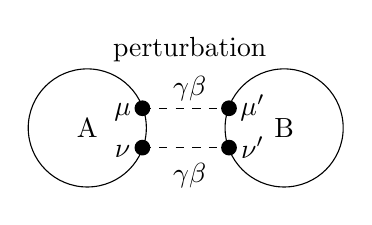
\begin{tikzpicture}
\draw (2,2) circle (0.75);
\draw (4.5,2) circle (0.75);
\fill[black] (2.7,2.25) circle (0.1);
\fill[black] (2.7,1.75) circle (0.1);
\fill[black] (3.8,2.25) circle (0.1);
\fill[black] (3.8,1.75) circle (0.1);
\draw[dashed] (2.7,2.25) -- (3.8,2.25);
\draw[dashed] (2.7,1.75) -- (3.8,1.75);
\node at (2.45,2.2) {$\mu$};
\node at (2.45,1.7) {$\nu$};
\node at (4.1,2.25) {$\mu'$};
\node at (4.1,1.75) {$\nu'$};
\node at (2,2) {A};
\node at (4.5,2) {B};
\node at (3.3,3.0) {perturbation};
\node at (3.3,2.5) {$\gamma\beta$};
\node at (3.3,1.4) {$\gamma\beta$};
\end{tikzpicture}
\end{center}

Assuming again that each pair of orbitals interacts with a term equal to $\gamma \beta$, we can write
\begin{equation}
\begin{split}
\braket{\chi_\mu | \hat{h}'| \chi_{\mu'}} = \gamma \beta, \\
\braket{\chi_\nu | \hat{h}'| \chi_{\nu'}} = \gamma \beta.
\end{split}
\end{equation}



Each orbital $\psi_i^\mathrm{A}$ on A will be stabilized by the interaction with the unoccupied orbitals on B
\begin{equation}
\Delta E_i^{\mathrm{A},(2)} = \sum_{k \neq i}^\text{virtual B} \frac{|\braket{\psi^\mathrm{A}_i|\hat{h}'|\psi^\mathrm{B}_k}|^2}{\epsilon^\mathrm{A}_i - \epsilon^\mathrm{B}_k}.
\end{equation}
Similarly, an orbital $\psi_i^\mathrm{B}$ on B will be stabilized by the interaction with the unoccupied orbitals on A by an amount
\begin{equation}
\Delta E_i^{\mathrm{B},(2)} = \sum_{k \neq i}^\text{virtual B} \frac{|\braket{\psi^\mathrm{B}_i|\hat{h}'|\psi^\mathrm{A}_k}|^2}{\epsilon^\mathrm{B}_i - \epsilon^\mathrm{A}_k}.
\end{equation}
Now let us suppose that the most important contribution comes from the interaction of the HOMO on A with the LUMO on B. The numerator for this contribution is given by
\begin{equation}
\Delta E_\mathrm{HOMO}^{\mathrm{A},(2)} = \frac{|\braket{\psi^\mathrm{A}_{\mathrm{HOMO}}|\hat{h}'|\psi^\mathrm{B}_{\mathrm{LUMO}}}|^2}{\epsilon^\mathrm{A}_{\mathrm{HOMO}}- \epsilon^\mathrm{B}_{\mathrm{LUMO}}}.
\end{equation}
If we plug in the definition of these two orbitals we get for the numerator
\begin{equation}
\begin{split}
\braket{\psi^\mathrm{A}_{\mathrm{HOMO}}|\hat{h}'|\psi^\mathrm{B_{\mathrm{LUMO}}}} &=
\sum_{\rho\sigma} 
\braket{\chi_\rho|\hat{h}'|\chi_\sigma}
C_{\rho,\mathrm{HOMO}}^\mathrm{A} C_{\sigma,\mathrm{LUMO}}^\mathrm{B} \\
&=
\braket{\chi_\mu|\hat{h}'|\chi_{\mu'}}
C_{\mu,\mathrm{HOMO}}^\mathrm{A} C_{\mu',\mathrm{LUMO}}^\mathrm{B}
+\braket{\chi_\nu|\hat{h}'|\chi_{\nu'}}
C_{\nu,\mathrm{HOMO}}^\mathrm{A} C_{\nu',\mathrm{LUMO}}^\mathrm{B}
\\
&=
\gamma\beta \underbrace{(
C_{\mu,\mathrm{HOMO}}^\mathrm{A} C_{\mu',\mathrm{LUMO}}^\mathrm{B}
+
C_{\nu,\mathrm{HOMO}}^\mathrm{A} C_{\nu',\mathrm{LUMO}}^\mathrm{B}
)}_{\delta}
=
\gamma\beta\delta
\end{split}
\end{equation}
We can now use this result to analyze the cyclization reaction between two molecules.

\section{Cyclization Reaction Between Two Molecules}
Consider the case of the HOMO of butadiene interacting with the LUMO of ethylene. In this case we can use simple symmetry considerations to learn something about the interaction of these two molecules in a cyclization reaction. The following plot show the HOMO and LUMO of butadiene and ethylene

\begin{center}
\includegraphics[width=3in]{../huckel/c2_cyclization_1.png}
\end{center}

For butadiene (A) the HOMO is antisymmetric, that is, it takes values with opposite signs on the two interacting atoms
\begin{equation}
C_{\mu,\mathrm{HOMO}}^\mathrm{A} = -C_{\nu,\mathrm{HOMO}}^\mathrm{A}
\end{equation}
and this is also true for the LUMO of ethylene (B)
\begin{equation}
C_{\mu',\mathrm{LUMO}}^\mathrm{B} = -C_{\nu',\mathrm{LUMO}}^\mathrm{B}.
\end{equation}
Taking these results into considerations we obtain
\begin{equation}
\delta = C_{\mu,\mathrm{HOMO}}^\mathrm{A} C_{\mu',\mathrm{LUMO}}^\mathrm{B}
+
C_{\nu,\mathrm{HOMO}}^\mathrm{A} C_{\nu',\mathrm{LUMO}}^\mathrm{B}
= 
2 C_{\mu,\mathrm{HOMO}}^\mathrm{A} C_{\mu',\mathrm{LUMO}}^\mathrm{B}
\end{equation}
This interaction leads to a lowering in energy since ${\epsilon^\mathrm{A}_{\mathrm{HOMO}}- \epsilon^\mathrm{B}_{\mathrm{LUMO}}} < 0$, therefore, we say that this interaction is \textbf{allowed}.
In general, the interaction of orbitals with the same symmetry is allowed.
For example, the interaction of the butadiene LUMO with the ethylene HOMO (the opposite of what we considered above) is a case where both orbitals are symmetric since
\begin{equation}
C_{\mu,\mathrm{LUMO}}^\mathrm{A} = C_{\nu,\mathrm{LUMO}}^\mathrm{A},
\end{equation}
and
\begin{equation}
C_{\mu',\mathrm{HOMO}}^\mathrm{B} = C_{\nu',\mathrm{HOMO}}^\mathrm{B}.
\end{equation}
For this case the quantity $\delta$ is also nonzero
\begin{equation}
\delta = 2 C_{\mu,\mathrm{LUMO}}^\mathrm{A} C_{\mu',\mathrm{HOMO}}^\mathrm{B}
\end{equation}

The interaction of two ethylene molecules is an example where the HOMO and LUMO have different symmetry

\includegraphics[width=3in]{../huckel/c2_cyclization_2.png}

In this case since
\begin{equation}
C_{\mu,\mathrm{HOMO}}^\mathrm{A} = C_{\nu,\mathrm{HOMO}}^\mathrm{A},
\end{equation}
and
\begin{equation}
C_{\mu',\mathrm{LUMO}}^\mathrm{B} = - C_{\nu',\mathrm{LUMO}}^\mathrm{B}.
\end{equation}
we find that $\delta = 0$.
This means that the interaction between orbitals of different symmetry is \textbf{forbidden}.
For general polyenes one has the following result:
\begin{equation}
(4n + 2) + (4n') \rightarrow 4 n'' + 2 \quad \text{symmetry allowed},
\end{equation}
while
\begin{equation}
\begin{split}
(4n + 2) + (4n' + 2) & \rightarrow 4 n'' +4\quad \text{forbidden}, \\
(4n) + (4n') & \rightarrow 4 n''\quad \text{forbidden}.
\end{split}
\end{equation}


\section{Orbital mixing rules}
Let's consider two atomic orbitals $\psi_i$ and $\psi_j$ and let them interact by, for example, bringing them together.
The interacting orbitals may be described by a two by two matrix of the form
\begin{equation}
\mathbf{h} = 
\begin{pmatrix}
\braket{\psi_i | \hat{h} |\psi_i} & \braket{\psi_i | \hat{h} |\psi_j} \\
\braket{\psi_j | \hat{h} |\psi_i} & \braket{\psi_j | \hat{h} |\psi_j}
\end{pmatrix}
=
\begin{pmatrix}
\epsilon_i & v \\
v & \epsilon_j
\end{pmatrix}.
\end{equation}

By examining the properties of the eigenvalues/eigenvectors of this matrix we can deduce some useful rules that can help us predict how orbitals mix.

\begin{itemize}
\item \textbf{Rule 1}. A pair of orbitals with zero overlap (orthogonal) do not mix. This is the case $v=0$, which basically means that the two orbitals do not interact due to symmetry.

\includegraphics[width=3in]{../huckel/c2_mix_rule_1.png}

\item \textbf{Rule 2}. When a pair of orbitals interact, they form a bonding (in-phase) orbital and an anti-bonding (out-of-phase) orbital. The bonding orbital is lower in energy than the antibonding orbital.

\includegraphics[width=2in]{../huckel/c2_mix_rule_2.png}

This rule follows from the equation for the eigenvalues of $\mathbf{h}$
\begin{equation}
\lambda_\pm = \frac{1}{2} (\epsilon_i + \epsilon_j)
\pm \frac{1}{2} \sqrt{(\epsilon_i - \epsilon_j)^2 + 4 v^2}.
\end{equation}
%Suppose $\epsilon_i \geq \epsilon_j$,
%The lowest eigenvalue ($\lambda_-$) corresponds to the eigenvector
%\begin{equation}
%v_1 = (\frac{\epsilon_i-\epsilon_j - \sqrt{(\epsilon_i - \epsilon_j)^2 + 4 v^2} }{2v} ,1)
%\end{equation}

\item \textbf{Rule 3}.  When the energy difference between a pair of orbitals before mixing is small and/or the overlap between a pair of orbitals is large, the energy separation becomes large after mixing.

\includegraphics[width=4in]{../huckel/c2_mix_rule_3.png}

\item \textbf{Rule 4}.  When a pair of orbitals with different energies interact, the newly formed MO has large contribution of the original orbital whose energy is closest to the newly formed MO.

\begin{center}
\includegraphics[width=4in]{../huckel/c2_mix_rule_4.png}
\end{center}


\item \textbf{Rule 5}. The same number of new MOs are created from the original orbitals before mixing ($N$ MOs from $N$ AOs).

\item \textbf{Rule 6}.    Suppose another orbital $\chi_c$ affects the two orbitals $\phi_1$  and $\phi_2$, which were formed mainly by interacting two orbitals $\chi_a$ and $\chi_b$.   The perturbation caused by the third orbital $\chi_c$ causes a small change of the orbital shape of $\phi_1$ and $\phi_2$.   When the energy of $\chi_c$ is higher than the energies of $\phi_1$ and $\phi_2$, the mixing of $\chi_c$ with $\phi_1$ and $\phi_2$ is in-phase.   When the energy of $\chi_c$ is lower than the energies of $\phi_1$ and $\phi_2$, the mixing of $\chi_c$ into $\phi_1$ and $\phi_2$ is out-of-phase.
 When three orbitals are interacting, the newly formed three MO's can be expressed with a linear combination of the original three orbitals.   The mixing coefficients depend on the energies of the original three orbitals.

\begin{center}
\includegraphics[width=4in]{../huckel/c2_mix_rule_6.png}
\end{center}
\end{itemize}


\section{Examples and Problems}
\subsection{Molecular orbitals of \ce{H3}}
Let us construct the molecular orbitals for the triangular and linear \ce{H3} species from the hydrogen atom and the molecular orbital of the \ce{H2} molecule. 

\textbf{Triangular \ce{H3}}

\begin{center}
\includegraphics[width=3in]{../huckel/c2_h3_tri.png}
\end{center}

 In the case of triangular \ce{H3}, let us assume that atomic hydrogen approaches on the bisecting axis of the hydrogen molecule.
 Note that $\chi_a$ interacts only with $\chi_b$ since the symmetry of $\chi_c$ is such that no mixing happens.
 The newly formed molecular orbital $\psi_1$ is the bonding combination between $\chi_a$ and $\chi_b$, and the molecular orbital $\psi_2$ is the corresponding anti-bonding combination. $\psi_3$ is the original $\chi_c$. 

\textbf{Linear \ce{H3}} (\ce{H. . . H-H})

\begin{center}
\includegraphics[width=3in]{../huckel/c2_h3_lin.png}
\end{center}

In the linear form of \ce{H3}, an hydrogen atom approaches the molecular axis of the hydrogen molecule.   The situation becomes different from the triangular \ce{H3} case, because all orbitals $\chi_a$, $\chi_b$, and $\chi_c$  interact with each other.
Comparing these two cases, we predict that the hydrogen exchange reaction \ce{H2 + H} prefers the linear transition-state structure since orbital interactions lead to an overall stabilization of the energy.

\begin{problem}[Molecular orbitals of \ce{H4}]
Construct the molecular orbitals for square \ce{H4} and linear \ce{H4} species from the two sets of molecular orbitals of the \ce{H2} molecule. 
Draw the orbital energy diagrams and discuss which structure is more stable.

\begin{center}
\includegraphics[width=2in]{../huckel/c2_problem_h4.png}
\end{center}

\end{problem}

\begin{problem}[$\pi$ MOs of benzene]
Create the six $\pi$-molecular orbitals of benzene by combining the two sets of $\pi$-orbitals of the allyl radical.   The picture shows only one side of $\pi$-plane (top view).

\begin{center}
\includegraphics[width=3in]{../huckel/c2_problem_benzene.png}
\end{center}

\end{problem}

%Once you know all the $\pi$-molecular orbitals of benzene, you can construct any -orbital of substituted benzene.   Let us make the HOMO (highest occupied molecular orbital) of phenol from benzene and the oxygen atom.
%   Assuming that the oxygen atom approaches to one of the carbon atoms of benzene along the C2v axis.   Before we construct the MOs of phenol, we should assign all of the unperturbed MOs under the C2v symmetry.   The MO of benzene does not interact with 2p-orbital of oxygen atom unless the symmetry of -MOs of benzene is b1 symmetry.   The HOMO of phenol 4 must be constructed from the anti-bonding combination between HOMO of the benzene 3 and the oxygen p-orbital o.   The second contributing orbital to the HOMO of phenol is the LUMO of benzene 5 which has a bonding combination with the oxygen p-orbital o.   We can neglect all other contributions from benzene -MO qualitatively, because the energy difference between 4 and 1 or 6 is larger than that between 4 and 3 or 5. 


 

 



\end{document}